\chapter{Реализация и экспериментальная проверка}

\begin{annotation}
	В данной главе приводятся детали разработки и экспериментальной проверки
	разработанной системы. Описан выбор инструментов, используемых для реализации
	программного обеспечения. Приводится выбор инфраструктурных решений,
	с учетом поставленных ранее системных и функциональных требований.
	Описаны состав и структура реализованного программного обеспечения.
\end{annotation}


% todo можно привести таблицу AKAIKE с разными гиперпараметрами для


\section{Выбор инструментальных средств}
\begin{annotation}
	В данном разделе обосновывается выбор инструментальных средств с учетом выдвинутых в 3
	главе требований к системе. Рассматриваются инструменты для обработки и хранения данных,
	для разработки backend и frontend части приложения. Рассматриваются инструменты для работы
	с нейросетями и графами для реализации компонента, связанного с вычислением нейро-нечеткой системы.
\end{annotation}



\section{Состав и структура реализованного программного обеспечения}
\begin{annotation}
	В данном разделе рассматривается состав и структура реализованного программного обеспечения.
	Приводятся характеристики разработанного программного продукта, возможности конфигурации отдельных
	компонент системы. Описано назначение исполняемых файлов, описаны требования к системному окружению.
\end{annotation}

Реализованное по --- это модуль на python.
Нужно прикрутить автотесты, coverage, линтеры

\section{Анализ данных}

\section{Построение модели}

\section{Тестирование разработанной системы}

Для тестирования системы были построены 3 варианта карты:
\begin{itemize}
	\item Карта без связей.
	\item Полносвязная карта.
	\item Карта с осмысленными связями.
\end{itemize}

Все карты обучались 100 эпох, имели размерность скрытого состояния 100,
количество исторических данных, обрабатываемых с помощью LSTM на одной итерации -~ 100.
Так же как и количество данных на выходе, сгенерированных.

% todo таблица
% Время обучения
% Качество

Карта без связей \ref{lstmfcm_empty}, обученная на тестовых данных
показала отличный результат для $ x_1, x_2, x_3, x_4  $. Однако ошибка
для $ x_5, y $ довольно велика. Такие предсказания эквивалентны предсказаниям
отдельно взятых моделей LSTM, обученных для предсказания временного ряда
по истории только этого временного ряда.

Карта, которая представляет из себя полносвязный граф \ref{pic:lstmfcm_fc},
из-за избыточности связи получила предсказания для $ x_1, x_2, x_3 $ даже
хуже, чем карта без связей. Это можно объяснить излишней сложностью модели.
Модель слишком усложнена и не может обучиться за заданное количество эпох.

Карте с осмысленными связями \ref{lstmfcm_meaningful} удалось сохранить качество
предсказаний для $ x_1 --- x_4 $ таким же, как и у карты без связей.
А так же удалось получить улучшение предсказания для $ y $.
Неожиданный результат получили для $ x_5 $. todo как так?

Для карт, у которых были связи с $ x_5, y $ получилось лучше предсказать значения
для этих рядов. Потому что значения этих рядов зависят от $ x_1 --- x_4 $.

Кроме того, на долгосрочных предсказаниях видно, что $ x_4 $ имеет проседания.
Вероятно, это связано с ограничениями, рассмотренными во второй главе.
Так как модель обучается на одних данных, а после предсказания, модель возвращает
данные в новой области значений, будущие предсказания становятся все более нестабильными.
todo не понятно, почему их нет на предсказании LSTM

\def\figurename{Рис}
\begin{figure}
	\centering
	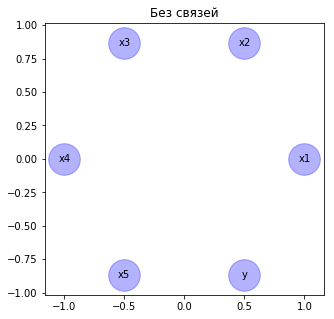
\includegraphics[width=0.7\columnwidth]{./img/lstmfcm_empty.png}
	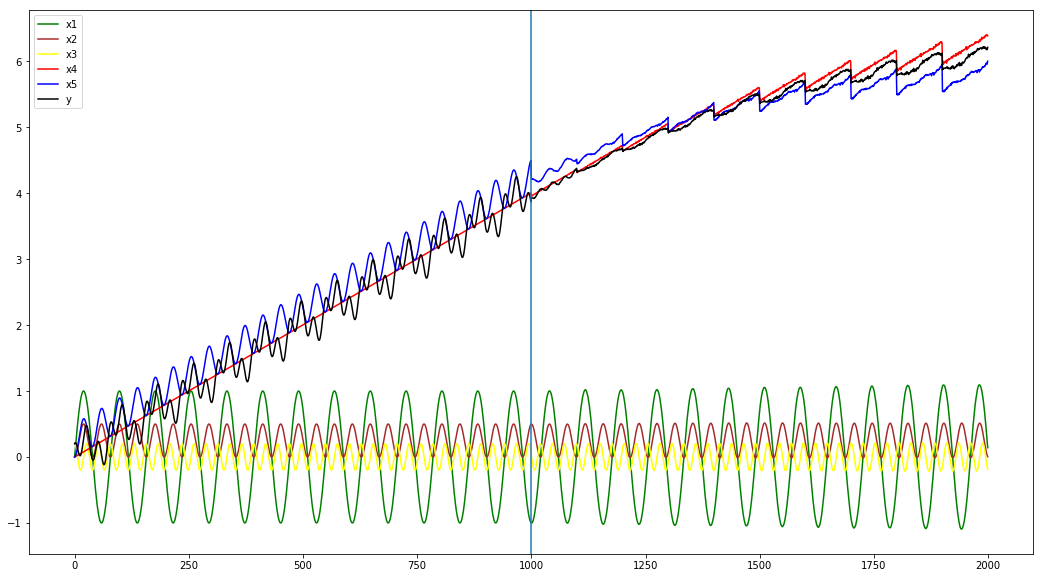
\includegraphics[width=0.9\columnwidth]{./img/lstmfcm_empty_prediction.png}
	\caption{Карта без связей концептов}
	\label{pic:lstmfcm_empty}
\end{figure}

\begin{figure}
	\centering
	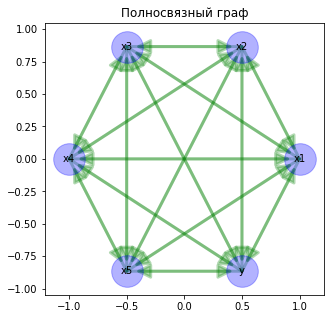
\includegraphics[width=0.7\columnwidth]{./img/lstmfcm_fc.png}
	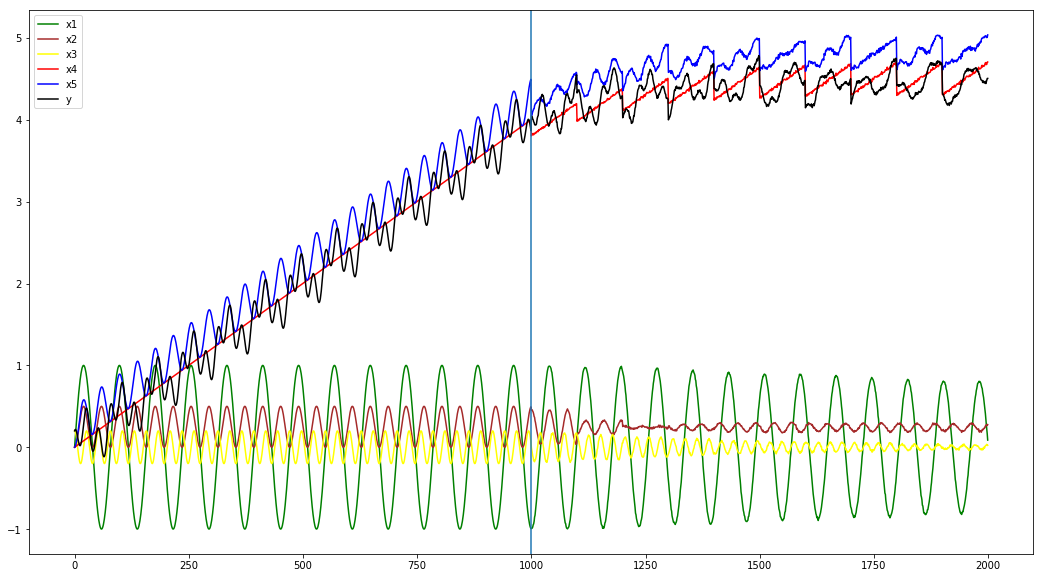
\includegraphics[width=0.9\columnwidth]{./img/lstmfcm_fc_prediction.png}
	\caption{Полносвязная карта}
	\label{pic:lstmfcm_fc}
\end{figure}

\begin{figure}
	\centering
	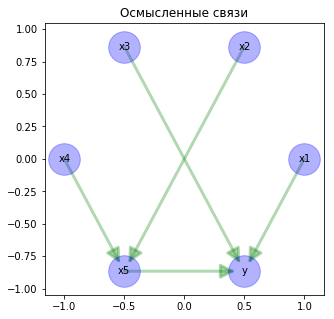
\includegraphics[width=0.7\textwidth]{./img/lstmfcm_meaningful.png}
	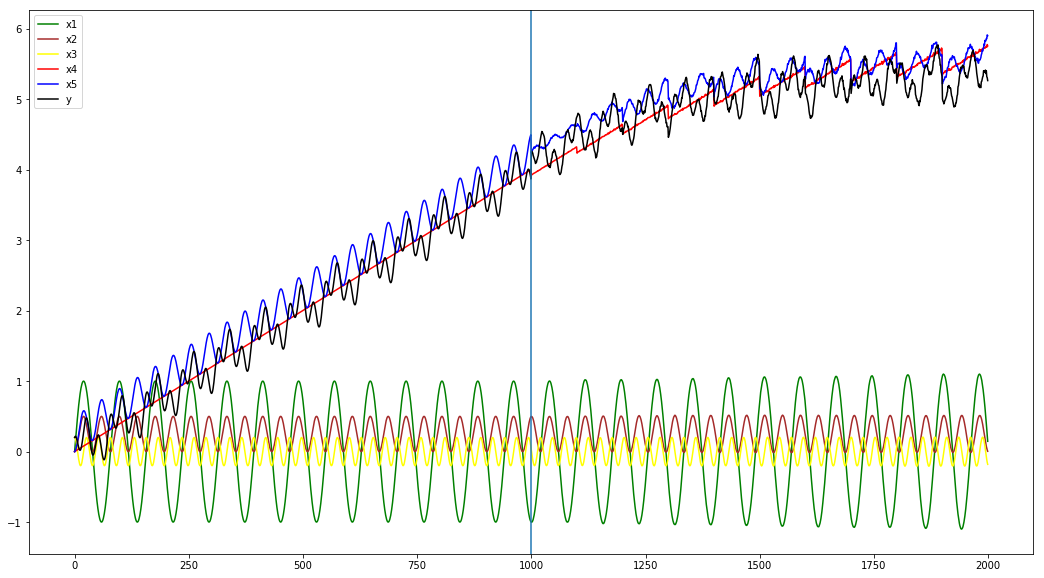
\includegraphics[width=0.9\textwidth]{./img/lstmfcm_meaningful_prediction.png}
	\caption{Карта с осмысленно расставленными связями}
	\label{pic:lstmfcm_meaningful}
\end{figure}


\section{Экспериментальное сравнение разработанной системы с существующими}

Была построена модель, основанная на LSTM,
которая одновременно анализирует все временные ряды тестовых данных.

Результат предсказаний такой модели представлен на рисунке \ref{lstm_only_prediction}.
Результат зашумлен по сравнению с предсказаниями карты (todo не могу объяснить).
И в отличие от карты, даже с осмысленными связями, на этом предсказании не наблюдается скачков
между итерациями предсказаний. И $ x_5 $ тоже удалось предсказать относительно успешно.

Данная модель так же, как и карта работала рекурсивно:
на каждой следующей итерации обрабатывала данные, полученные на предыдущей.
Скачок вначале предсказаний, скорее всего, связан с тем, что после обучения,
скрытое состояние сети выставляется заново, так как меняется его размерность.
Возможно, использование скрытого состояния одинаковой размерности во время
тренировки и во время тестирования, может избавить от этой проблемы. Однако
в LSTM NFCM между итерациями тоже сохраняются эти скачки, хотя между итерациями
скрытое состояние не переинициализируется.

\begin{figure}
	\centering
	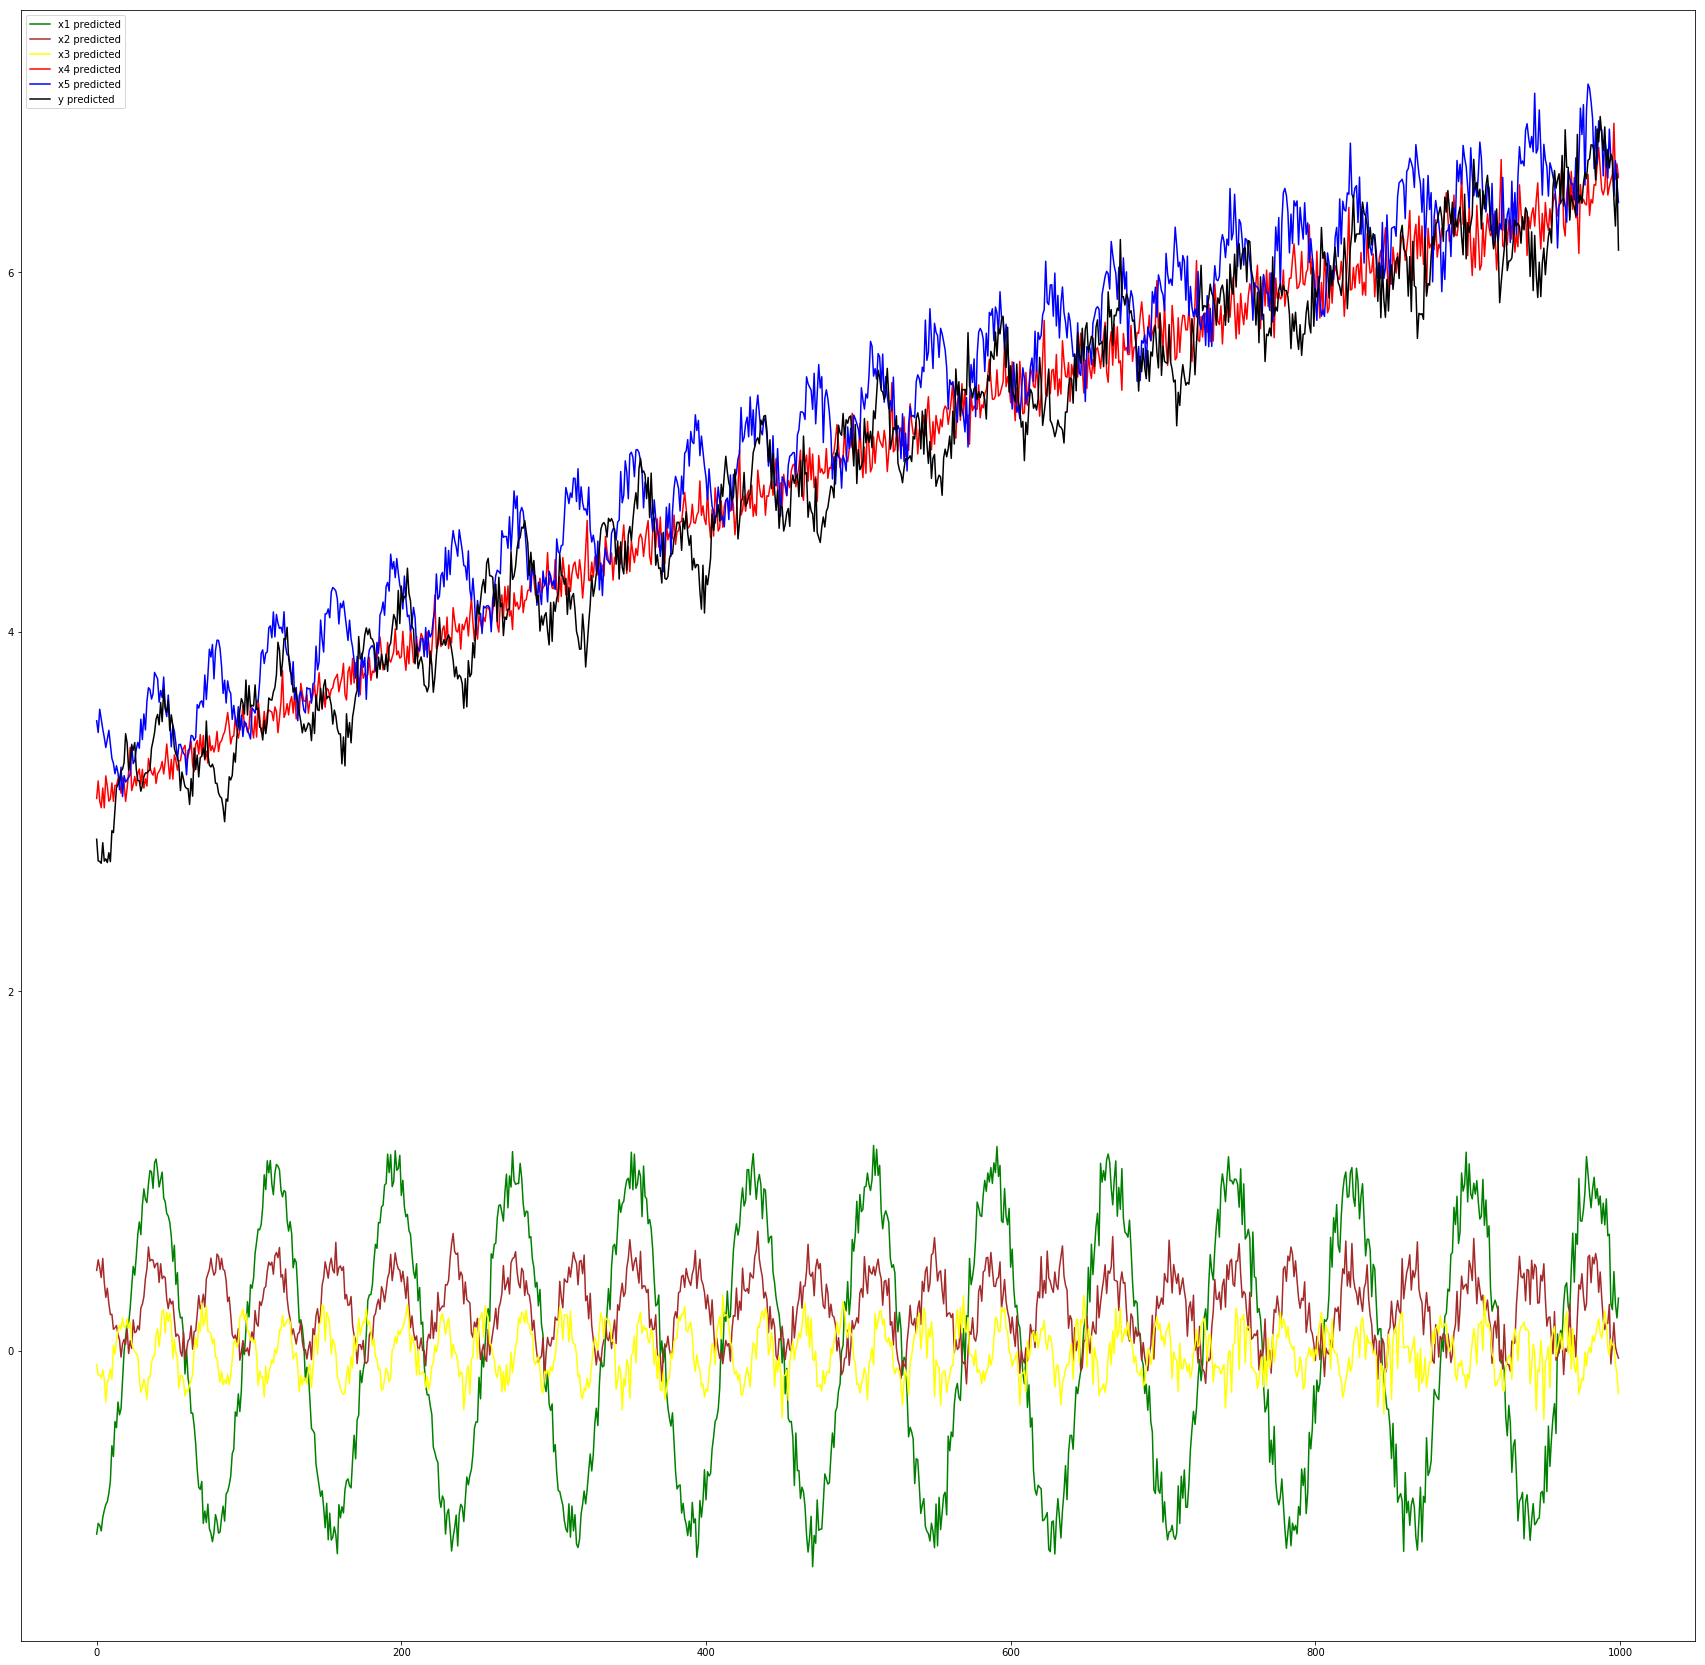
\includegraphics[width=0.9\textwidth]{./img/lstm_only_prediction.png}
	\caption{LSTM only model prediction}
	\label{pic:lstm_only_prediction}
\end{figure}


Вторая модель была построена только с использованием ARIMAX модели.
Параметры модели подбирались на кросс-валидации. Была выбрана модель с минимальным
значением критерия Акаике. Гиперпараметры $ p $, $ q $ пробегали значения от 0 до 7.
Гиперпараметр $ d $ -- от 0 до 1. Всего получилось 192 набора гиперпараметров.

В результате эксперимента оптимальной моделью оказалась $ ARIMA(5, 1, 5) $.
Значение критерия Акаике для данной модели было минимальным -~ $ AIC: 6231.963732352154 $





После этого была построена коррелограмма исследуемого ряда и определены оптимальные
значения 

\section{Влияние гиперпараметров модели на качество предсказаний}

% todo
% Посмотреть, как карта будет самобалансироваться, если сделать прикольную обратную связь.

При уменьшении количества эпох обучения, карта может расходиться, даже карта с осмысленными связями.

Увеличение параметра $ n\_steps\_in $, количество предыдущих значений временных рядов,
а так же размерность скрытого состояния увеличивают количество требуемой для обучения
памяти не более, чем линейно каждый. Конкретный показатель роста будет зависеть от
плотности связей в карте.
Уменьшение этих параметров, позволяет сэкономить память и ускорить обучение,
но страдает качество предсказаний.


\section{Моделирование с помощью разработанной системы}
\begin{annotation}
	В данном разделе описывается процесс тестирования разработанной системы.
	Описаны реализованные unit-тесты и описывается процесс функционального тестирования.
	Приводятся результаты моделирования. Проверяется то, что система соответствует выдвинутым ранее требованиям.
	Производится оценка работы системы.
\end{annotation}

\section{Выводы}

В данной главе была реализована система для автоматического когнитивного картирования с использованием
методов нейронных сетей.
Также описаны инструменты, с помощью которых была реализована система.
Описана структура программного обеспечения, проведено тестирование разработанной системы.
На основе тестирования была дана оценка реализованной системе.

% Следует перечислить, какие практические результаты были получены, а именно: какое программное или иное обеспечение было создано. В число результатов могут входить, например, методики тестирования, тестовые примеры (для проверки корректности/оценки характеристик тех или иных алгоритмов) и др. По каждому результату следует сделать вывод, насколько он отличается от известных промышленных аналогов и исследовательских прототипов.

